\begin{frame}{Der \raspberry Default}{\cod{HDMI}, \cod{USB}}
 \begin{itemize}
  \item Speisung per \cod{USB} vom Host
  \item Bildschirm per \cod{HDMI}
  \item Tastatur per \cod{USB}
 \end{itemize}

 \begin{block}{Vorteil}
  \begin{itemize}
  \item der Standard 
  \end{itemize} 
 \end{block}

 \begin{block}{Nachteil}
 \begin{itemize}
  \item braucht Bildschirm/Tastatur
  \begin{itemize}
  \item nicht so viele vorhanden
  \end{itemize}
 \end{itemize}
 \end{block}
\end{frame}

\subsection{Via Netzwerk}
\begin{frame}{Via Netzwerk/Ethernet}{\cod{ssh}}
 \begin{itemize}
  \item Speisung via \cod{USB} vom Host
  \item Verbindung zum Target via \cod{ssh}
 \end{itemize}
  \begin{block}{Vorteil}
  \begin{itemize}
  \item braucht keinen Bildschirm/Tastatur
  \end{itemize} 
 \end{block}
 \begin{block}{Nachteil}
  \begin{itemize}
   \item etwas komplexere Konfiguration
   \begin{itemize}
    \item vor allem im Schulnetz
   \end{itemize}
  \end{itemize} 
 \end{block}
 \remark{Ist aber unser Ziel}
\end{frame}

\begin{frame}{Die Tools}{f�r die Verbindung}
 \begin{itemize}
  \item \cod{wireshark} f�r die Netz�berwachung
  \item \cod{nmap} f�r Portscans
  \item \cod{ifconfig} f�r die Netzschnittstelle
  \item Ein DHCP Server z.B. \cod{dnsmasq}
 \end{itemize}
 \see{net-setup.txt}
\end{frame}

\begin{frame}{Lokales Netzwerk}{Host $\to$Target}
 \begin{description}
  \item[Host] DHCP Server
  \item[Target] Mit dem Host verbunden
 \end{description}
\end{frame}

\begin{frame}{Via Schulnetz}
 \begin{itemize}
  \item einfach einstecken
 \end{itemize}
\end{frame}

\begin{frame}{Konfiguration \cod{SSH}}{Server}
 \begin{itemize}
  \item \cod{ssh-keygen -t{\em type} -f /etc/ssh/ssh\_host\_{\em type}\_key}
  \begin{itemize}
   \item mit \cod{{\em type}=rsa\textbar dsa}s
  \end{itemize}
  \remark{Auf dem {\em Target}}
 \end{itemize}
 
\end{frame}

\subsection{RS232}
\begin{frame}{\cod{RS232}}{Adapter \cod{RS232}$\to$\cod{USB}: die direkteste Verbindung}
 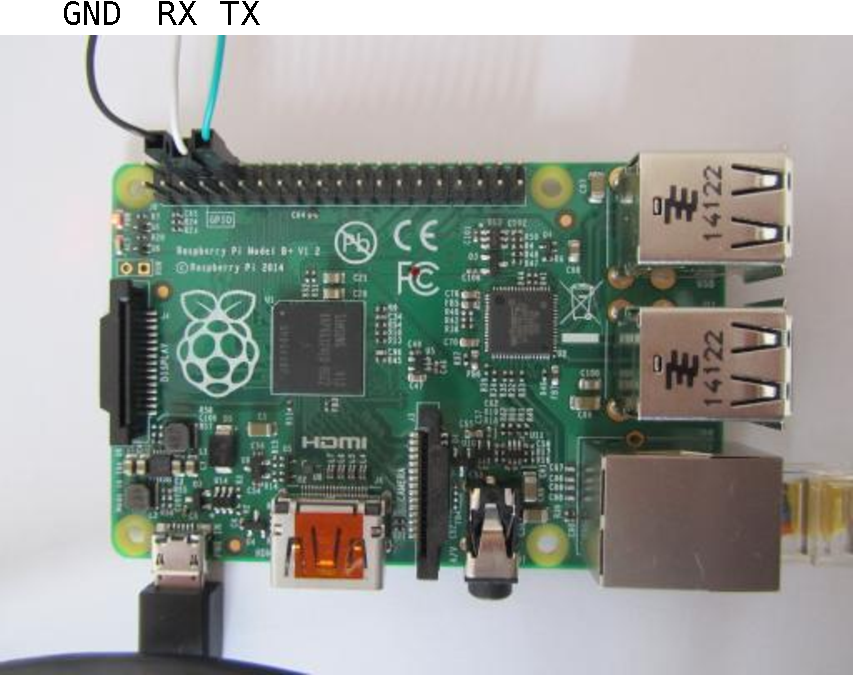
\includegraphics[width=8cm]{board.pdf}
 \begin{textblock}{150}(90,50)
  \begin{itemize}
   \item 115200 Baud
   \item 8N1
   \item no handshake
  \end{itemize}
 \end{textblock}
\end{frame}
